\begin{figure}[h]
\centering 
\includegraphics[scale=1]{images/mongoPic.png}
\caption{MongoDB logo}
\end{figure}
\noindent MongoDB is a cross-platform, document oriented database that provides, high performance, high availability, and easy scalability. MongoDB works on concept of collection and document.

Database is a physical container for collections. Each database gets its own set of files on the file system. A single MongoDB server typically has multiple databases.

Collection is a group of MongoDB documents. It is the equivalent of an RDBMS table. A collection exists within a single database. Collections do not enforce a schema. Documents within a collection can have different fields. Typically, all documents in a collection are of similar or related purpose.

A document is a set of key-value pairs. Documents have dynamic schema. Dynamic schema means that documents in the same collection do not need to have the same set of fields or structure, and common fields in a collection's documents may hold different types of data.

\begin{figure}[h]
\centering 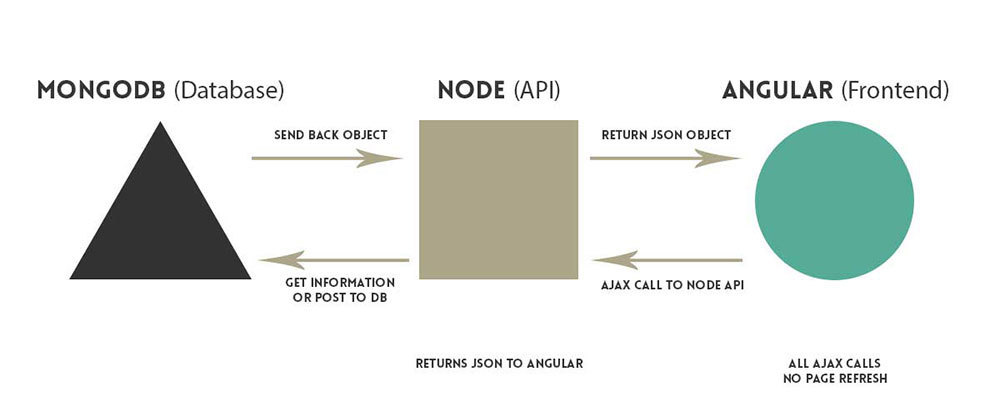
\includegraphics[scale=1]{images/mongodb.jpg}
\caption{Mean Model}
\end{figure}

\subsection{Advantages of MongnoDB}
\begin{itemize}
\item Schema less − MongoDB is a document database in which one collection holds different documents. Number of fields, content and size of the document can differ from one document to another.
\item Deep query-ability. MongoDB supports dynamic queries on documents using a document-based query language that's nearly as powerful as SQL.
\item Uses internal memory for storing the (windowed) working set, enabling faster access of data.
\item Conversion/mapping of application objects to database objects not needed.
\end{itemize}

\subsection{Why to use MongnoDB}
\begin{itemize}
\item Document Oriented Storage − Data is stored in the form of JSON style documents.
\item Index on any attribute.
\item Replication and high availability.
\item Auto-sharding
\end{itemize}

\subsection{Where to use MongnoDB}
\begin{itemize}
\item Big Data
\item Content Management and Delivery
\item Mobile and Social Infrastructure
\item User Data Management
\end{itemize}

\subsection{Installation of MongoDB}
Doxygen can be installed using following commands:\\

\hspace{4pt} \$ sudo apt-key adv --keyserver hkp://keyserver.ubuntu.com:80 --recv 0C49F3730359A14518585931BC711F9BA15703C6

\hspace{4pt} \$ sudo apt-get update

\hspace{4pt} \$ sudo apt-get install -y mongodb-org

\hspace{4pt} \$ sudo service mongod start
